\documentclass[a4paper]{article}
\usepackage[pdftex]{graphicx}
\usepackage[utf8]{inputenc}
\usepackage{enumerate}
\usepackage{siunitx}
\sisetup{locale=DE}
\usepackage{icomma}
\usepackage{amssymb}
\usepackage{tikz}
\usepackage{href-ul}
\hypersetup{
	colorlinks=true,
	linkcolor=blue,
	urlcolor=blue}
\usepackage{geometry}
\geometry{a4paper, top=15mm, left=15mm, right=15mm, bottom=15mm,
	headsep=10mm, footskip=12mm}

\begin{document}
	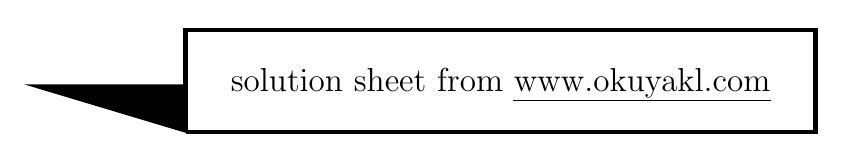
\begin{tikzpicture}(10,3)
		\draw[ultra thick](2,0) --(10,0) -- (10,1.3) --(2,1.3) -- (2,0);
		\draw[fill=black](2,0)-- (0,.6) -- (2,.6) -- (2,0);
		\node at (6,.6) {\large solution sheet from \href{http://www.okuyakl.com}{www.okuyakl.com}};
	\end{tikzpicture}
	\vspace{0.5 cm}
	
	\noindent {\bf task 1. a)}\\
	Let $M$ be the mass of Phobos, $m$ the mass of the sample to be accelerated, $G$ the gravitational constant and $R$ the radius of Phobos. According to the law of gravity:
	$$
	\renewcommand{\arraystretch}{2}
	\begin{array}{rcll}
		m\cdot g_{Ph} & = & { G \cdot M \cdot m \over R^2} & | :m \\
		g_{Ph} & = & { G \cdot M \over R^2} \\
		g_{Ph} & = & { \SI{6,67e-11}{{\meter^3} \over {\kilogram\second^2}} \cdot \SI{1,1e16}{\kilogram} \over (\SI{11000}{\meter})^2} \\
		g_{Ph} & = & \SI{6,1e-3}{\meter \over{ \second^2}}
	\end{array}
	$$
	\vspace{0.5 cm}
	
	\noindent {\bf task 1. b)}\\
	The ball is supposed to circle Phobos in a circular path near the surface. The balance of forces between centripetal force and gravitational force applies here:
	$$
	\renewcommand{\arraystretch}{2}
	\begin{array}{rcll}
		{m\cdot v^2 \over R} & = & { G \cdot M \cdot m \over R^2} & | :m \cdot R\\
		v^2 & = & { G \cdot M \over R} & \sqrt{\quad}\\
		v & = & \sqrt{ G \cdot M \over R} \\
		v & = & \sqrt{ \SI{6,67e-11}{{\meter^3} \over {\kilogram\second^2}} \cdot \SI{1,1e16}{\kilogram} \over \SI{11000}{\meter}} \\
		v & = & \SI{8,2}{\meter \over \second}
	\end{array}
	$$
	The ball should be thrown with a speed of $v=\SI{8,2}{\meter \over \second}$. (So don't throw it too hard, otherwise it will disappear into space!)
	\vspace{0.5 cm}
	
	\noindent {\bf task 1. c)}\\
	Let the circumference of the circular path be $U = 2 \pi \cdot R$. Then the required time is the same (remember: $s=v\cdot t$):
	$$t = {U \over v}= {2 \pi \cdot R \over v} = {2 \pi \cdot \SI{11000}{\meter} \over \SI{8,2}{\meter \over \second}}= \SI{8430}{\second} \approx \SI{2}{\hour}\SI{20}{\minute}$$
	The orbital period is very long at over two hours; So you should take something to read with you...
	
	\vspace{0.5 cm}
	
	\noindent{\bf Task 2. a)}\\
	\begin{itemize}
		\item Greater distance from the center of the earth means less attraction.
		\item There is no centrifugal force at the pole; it is maximum at the equator.
	\end{itemize}
	\vspace{0.5 cm}
	
	\noindent{\bf Task 2. b)}\\
	The formula for calculating $g$ can be derived using the law of gravity:
	$$
	\renewcommand{\arraystretch}{2}
	\begin{array}{rcll}
		m g &=& {G \cdot M \cdot m \over r^2} &|:m \\
		g &=& {G \cdot M \over r^2} \\
		g_{Pol} &=& {\SI{6.674e-11}{{\meter^3} \over {\kilogram\second^2}} \cdot\SI{5.972e24}{\kilogram} \over ({ \SI{6357e3}{\meter}})^2 }&=\SI{9,860}{\meter \over{ \second^2}}\\
		g_{Aeq}^* &=& {\SI{6.674e-11}{{\meter^3} \over {\kilogram\second^2}} \cdot\SI{5.972e24}{\kilogram} \over ({\SI{6378e3}{\meter}})^2 }&=\SI{9,798}{\meter \over{ \second^2}}\\
	\end{array}
	$$
	$g_{Aeq}^*$ is still without taking into account the centrifugal acceleration $a_z$; this still has to be subtracted to get $g_{Aeq}$:
	$$
	\renewcommand{\arraystretch}{2}
	\begin{array}{rcll}
		a_z &=& {\omega^2 r}\\
		&=& ({2 \pi \over 24 \cdot 60 \cdot \SI{60}{\second}})^2 \cdot \cdot\SI{6378e3}{\meter}\\
		&=& \SI{5,368e-3}{\meter \over{ \second^2}}
	\end{array}
	$$
	$$g_{Aeq} = g_{Aeq}^* - a_z = \SI{9,793}{\meter \over{ \second^2}}$$
	It should be noted that the effect of centrifugal force is much smaller than that of the difference in radius.
	The relative difference in gravitational accelerations is:
	$${g_{Pol}-g_{Aeq}\over g_{Pol}}=0.68\%$$
	\vspace{0.5 cm}
	
	\noindent{\bf Task 3.}\\
	We equate centrifugal force with gravitational force:
	$$
	\renewcommand{\arraystretch}{2}
	\begin{array}{rcll}
		{m v^2 \over r} &=& {G \cdot M \cdot m \over r^2} &|:m v^2 \cdot r^2 \\
		r &=& { G \cdot M \over v^2}\\
		r &=& { \SI{6.67e-11}{{\meter^3} \over {\kilogram\second^2}} \cdot 10 \cdot\SI{1.98e30}{\kilogram} \over (\SI{3,0e8}{\meter\over \second})^2} \\
		r &=& \SI{15e3}{\meter}
	\end{array}
	$$
	\vspace{0.5 cm}
	
	\noindent{\bf Task 4.}\\
	The mass of the Earth is $M_E$, that of the Moon is $M_M$.
	Let the distance of this point to the Earth be $d-r$. Then the following applies to the gravitational forces:
	$$
	\renewcommand{\arraystretch}{2}
	\begin{array}{rclll}
		F_{G,Earth} &=& F_{G,Moon} \\
		{G \cdot M_E \cdot m \over (d-r)^2} &=& {G \cdot M_M \cdot m \over r^2} \\
		{M_E\over (d-r)^2} &=& { M_M\over r^2} \\
		{M_E \over M_M} &=& {(d-r)^2 \over r^2} \\
		\sqrt{M_E \over M_M}&=& {d-r \over r} \\
		\sqrt{M_E \over M_M}&=& {d\over r}-1 \\
		r &=& { d \over \sqrt{M_E \over M_M}+1} &= {\SI{384400}{\kilo\meter} \over \sqrt {\SI{5.97e24}{\kilogram} \over\SI{7.35e22}{\kilogram}}+1}&=\SI {38400}{\kilo\meter}
		\end{array}
		$$
		\vspace{0.5 cm}
		
		\noindent{\bf Task 5. a)}\\
		The radius of its orbit is:
		$$ r = { v \cdot T \over 2 \pi}={\SI{3700}{\meter \over \second} \cdot 130\cdot \SI{60}{\second} \over 2 \pi } =\SI{4,6e6}{\meter}$$
		This means that the planet's radius is:
		$$R=r-\SI{800}{\kilo\meter} = \SI{3.8e6}{\meter} \approx \SI{3800}{\kilo\meter}$$
		\vspace{0.5 cm}
		
		\noindent{\bf Task 5. b)}\\
		We set gravity equal to centripetal force and solve for $M$:
		$$
		\renewcommand{\arraystretch}{2}
		\begin{array}{rclll}
		{m v^2 \over r} &=& G\cdot {M\cdot m \over r^2} \\
		M &=& {v^2 \cdot r \over G} &= {(\SI{3700}{\meter\over \second})^2 \cdot \SI{3,8e6}{\meter} \over \SI{6.67e-11}{{\meter^3}\over {\kilogram{\second^2}}}} & = \SI{9.4e23}{\kilogram}\\
		\end{array}
		$$
		
		This means it has almost a sixth of the mass of the Earth.
		\vspace{0.5 cm}
		
		\noindent{\bf Task 5. c)}\\
		We equate weight to gravity:
		$$
		\renewcommand{\arraystretch}{2}
		\begin{array}{rclll}
		mg &=& G\cdot {M\cdot m \over r^2} \\
		g&=& G\cdot {M\over r^2} &= \SI{6,67e-11}{{\meter^3} \over {\kilogram\second^2}} \cdot {\SI{9 .4e23}{\kilogram} \over (\SI{3.8e6}{\meter})^2 }&=\SI{4.34}{\meter \over {\second^2}}
		\end{array}
		$$
		
		\begin{center}
		\includegraphics[width=7 cm]{../../viecher/eendcomic.pdf}
		
		Here you can go back to the \href{https://www.okuyakl.de/phys/p10kreiL413/ae413.pdf}{task sheet}
		\end{center}
		
	\end{document}